\noindent Considering that $\Delta$Q$^{*}$ $=$ Q$^{*}_{rbc}$ $-$ Q$^{*}_{blood}$ against either the discharge haematocrit or branch diameter alone could not differentiate the RBC-depletion zone from the RBC-enrichment zone, haemodynamic indicators like Q$^{*}_{blood}$ was examined instead. Excluding one single outlier from Figure \ref{DisproportionalityIndexQblood} below, we have noticed that the differentiation between RBC-depletion and RBC-enrichment for each child branch can be determined with the fractional blood flow Q$^{*}_{blood}$ in the given child branch. This observation features a potential haemodynamic mechanism that may exist in the microvascular networks based on simulation data. For this reason, the time-averaged behaviour of RBC partitioning was considered (as shown in Figure \ref{TimeAveragedRBCPartitioningBehaviours}) to assess for the presence of the Zweifach-Fung effect.\cite{SVANES1968210, FUNG197334} The results show that majority of the investigated child branches have classical partitioning behaviour while only a small number of those branches have reverse partitioning behaviour. Hence, this demonstrated the presence of the Zweifach-Fung effect which describes the heterogeneous partitioning behaviour of RBC suspension for both child branches in each selected bifurcation across the networks. 

\begin{figure}[H]
\centering
\begin{subfigure}{0.48 \textwidth}
    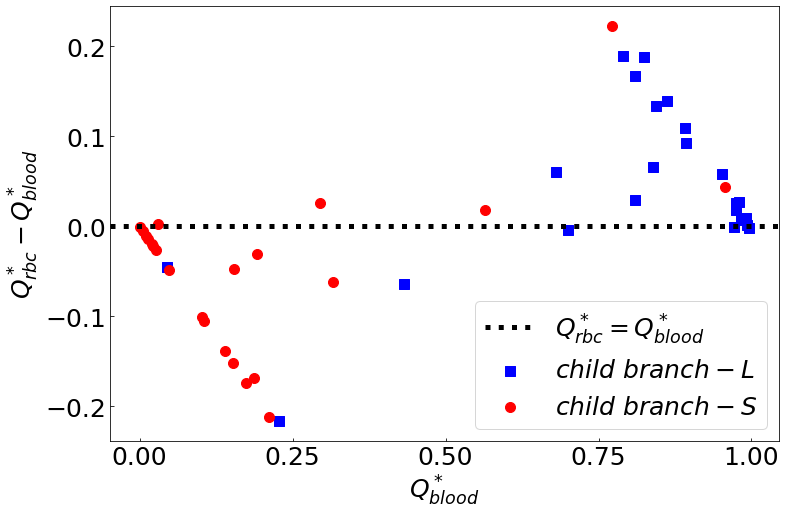
\includegraphics[width=1\textwidth]{images/DisproportionalityIndexQblood.png}
    \caption{\textit{Disproportionality Indices for all of the investigated child branches against normalised blood flow Q$^{*}$ across the networks} \label{DisproportionalityIndexQblood}}
\end{subfigure}
\hfill
\begin{subfigure}{0.48 \textwidth}
    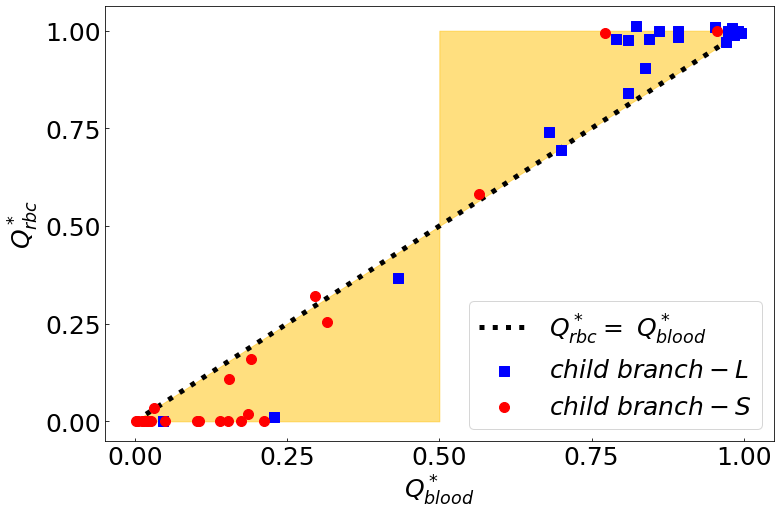
\includegraphics[width=1\textwidth]{images/TimeAveragedRBCPartitioningBehaviours.png}
    \caption{\textit{Time-averaged RBC Partitioning Behaviours found across the networks, Classical: 52 branches (yellow region) | Reverse: 5 branches (white region)} \label{TimeAveragedRBCPartitioningBehaviours}}
\end{subfigure}
\caption{\textit{Distinct correlation between $\Delta$Q$^{*}$ $=$ Q$^{*}_{rbc}$ $-$ Q$^{*}_{blood}$ and Q$^{*}_{blood}$ highlights a potential haemodynamic mechanism within the micro-vascular networks. Simulation data of Q$^{*}_{rbc}$ against Q$^{*}_{blood}$ distinguishes the different RBC partitioning behaviours occurring for the child branches within each bifurcation. The black dotted line represents a linear hypothesis for Q$^{*}_{blood}$ and Q$^{*}_{rbc}$ without the presence of plasma skimming.} \label{PlasmaSkimmingEffects}}
\end{figure}

\noindent In reference to these findings from simulation data, it does suggest to us the existence of plasma skimming effect occurring in the micro-vascular networks. For the purpose of validation, the simulation data at each diverging bifurcation was compared to the empirical predictions from the PSM model (Equations \ref{Pries_equation1}$-$\ref{Pries_equationX}).\cite{A.R.Pries2005Mbvi, PriesAR1990BFiM} The results indicated 17 out of 23 bifurcations show good agreement with predictions from PSM with errors of less than 5$\%$ (see Table \ref{ErrorsPSM} for complete error evaluation). An illustration of two exemplar bifurcations showing that the simulation data matched well with empirical predictions is presented in Figure \ref{DeviationsPSM}a$-$b. In the first bifurcation (Figure \ref{DeviationsPSM1}), both child branches have a substantial fraction of blood flow (approximately 30\% and 70\% in CB-S and CB-L respectively) with fractional RBC fluxes almost identical to PSM predictions. In the second bifurcation (Figure \ref{DeviationsPSM2}), the larger child branch has almost all of the RBCs (Q$^{*}_{rbc}$ $\approx$ 98\%) as it receives close to 90\% of the blood flow from the parent branch which leaves the smaller child branch with practically little blood flow and no RBCs. 

\begin{figure}[H]
\centering
\begin{subfigure}{0.48 \textwidth}
    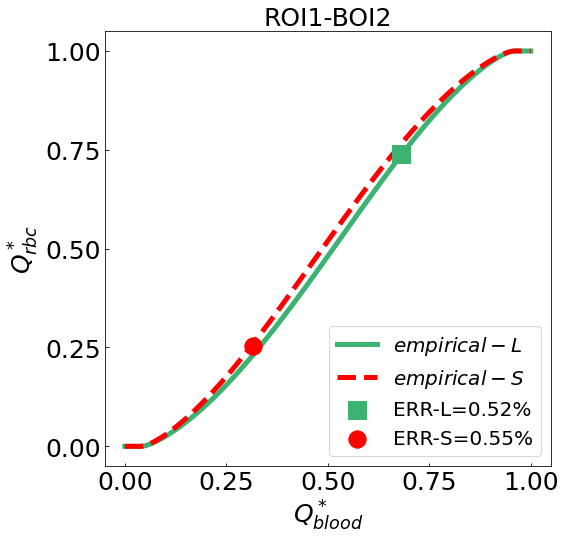
\includegraphics[width=0.92\textwidth]{images/DeviationsPSM1.png}
    \caption{\textit{Proportions of blood flow (Q$^{*}_{blood}$) in CB-L and CB-S are approximately 70\% and 30\% respectively} \label{DeviationsPSM1}}
\end{subfigure}
\hfill
\begin{subfigure}{0.48 \textwidth}
    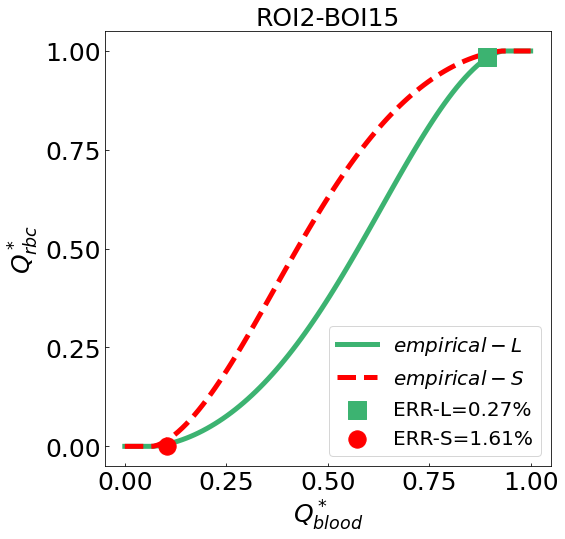
\includegraphics[width=0.92\textwidth]{images/DeviationsPSM2.png}
    \caption{\textit{Proportions of blood flow (Q$^{*}_{blood}$) in CB-L and CB-S are approximately 90\% and 10\% respectively} \label{DeviationsPSM2}}
\end{subfigure}
\hfill
\begin{subfigure}{0.48 \textwidth}
    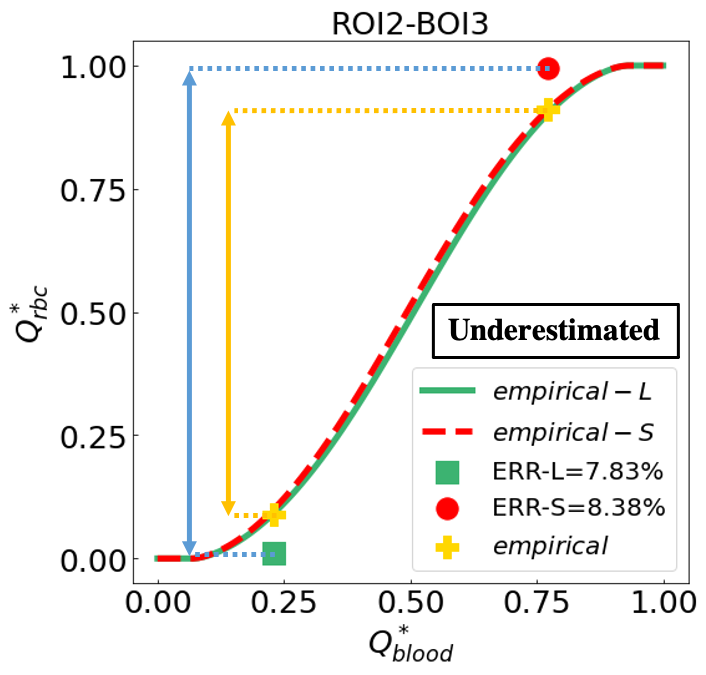
\includegraphics[width=0.92\textwidth]{images/DeviationsPSM3.png}
    \caption{\textit{PSM model slightly underestimated RBC flux comparison between the two child branches} \label{DeviationsPSM3}}
\end{subfigure}
\hfill
\begin{subfigure}{0.48 \textwidth}
    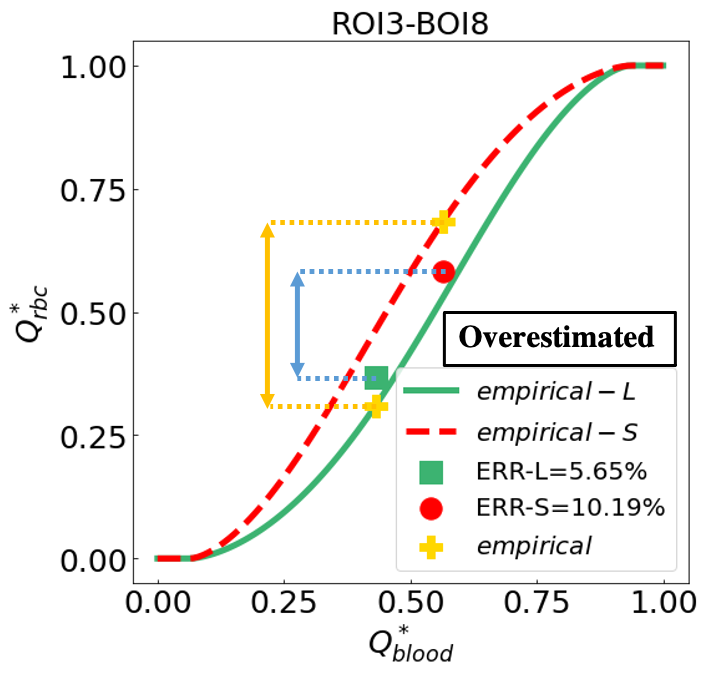
\includegraphics[width=0.92\textwidth]{images/DeviationsPSM4.png}
    \caption{\textit{PSM model considerably overestimated RBC flux comparison between the two child branches} \label{DeviationsPSM4}}
\end{subfigure}
\caption{\textit{Examples of good (a$-$b) and bad (c$-$d) matches of fractional RBC fluxes (Q$^{*}_{rbc}$) between simulation data (squares and circles) and the empirical predictions (solid lines and crosses) from Pries Phase Separation Model based on the given proportion of blood flows for both the "L" and "S" child branches in each selected bifurcation.} \label{DeviationsPSM}}
\end{figure}

\noindent For the remaining 6 of 23 bifurcations investigated, the simulated RBC fluxes have deviations of greater than 5\% against the PSM predictions, and two of such bifurcations are shown in Figure \ref{DeviationsPSM}c$-$d. The difference in RBC flux between the two child branches for the first bifurcation (Figure \ref{DeviationsPSM3}) marginally underestimated the PSM predictions while it is significantly overestimated for the second bifurcation (Figure \ref{DeviationsPSM4}). Such observations are found because of the asymmetric RBC distribution in the cross-sections of the parent branches which is opposed to the primary assumption of symmetrical haematocrit profile by the empirical model. Therefore, without the knowledge of the cross-sectional RBC distributions, it will be challenging to accurately predict the RBC perfusion in any given vascular network. \\

\noindent In consideration of the above findings, the Phase Separation Model developed by Pries et al.\cite{A.R.Pries2005Mbvi, PriesAR1990BFiM} attributed to the plasma skimming effect has appropriately described the RBC flux partitioning in 17 out of the 23 selected bifurcations. (see Figures \ref{DisproportionalityIndexQblood-ROI1}$-$\ref{DisproportionalityIndexQblood-ROI3} in the Appendix \ref{EvaluationOfSimulationDataVSPSM}) Therefore, this implies that the mechanism behind RBC enrichment/depletion within the studied networks is the plasma skimming effect. Also, this suggests that the RBC distribution within the micro-vascular network is flow-mediated instead of geometry-dominant.



\begin{table}[H]
\centering
\caption{\textit{Full evaluation of the deviations between simulation data and the empirical predictions from Pries Phase Separation Model. The "L"/"S" indicate the relatively larger and smaller child branches in each diverging bifurcation respectively.}
\label{ErrorsPSM}}
\scalebox{0.75}{
\begin{tabular}{*{11}{c}}
\dtoprule
\textbf{ROIs} & \textbf{CBs} & \textbf{BOI-2} & \textbf{BOI-7} & \textbf{BOI-9} & \textbf{BOI-10} & \textbf{BOI-11} & \textbf{BOI-13} & $-$ & $-$ & $-$ \\
\midrule[0.5pt]
\multirow{2}{*}{ROI-1} & CB-L & 0.52\% & 2.39\% & 0.68\% & 0.68\% & 0.0\% & 0.0\% & $-$ & $-$ & $-$ \\
& CB-S & 0.55\% & 4.3\% & 0.0\% & 0.0\% & 0.0\% & 0.0\% & $-$ & $-$ & $-$ \\
\dbottomrule
\textbf{ROIs} & \textbf{CBs} & \textbf{BOI-1} & \textbf{BOI-2} & \textbf{BOI-3} & \textbf{BOI-4} & \textbf{BOI-7} & \textbf{BOI-9} & \textbf{BOI-11} & \textbf{BOI-12} & \textbf{BOI-15} \\
\midrule[0.5pt]
\multirow{2}{*}{ROI-2} & CB-L & 2.32\% & 0.58\% & 7.83\% & 8.11\% & 0.05\% & 1.34\% & 5.36\% & 0.99\% & 0.27\% \\
& CB-S & 4.61\% & 0.0\% & 8.38\% & 8.2\% & 0.06\% & 3.16\% & 3.98\% & 0.0\% & 1.6\% \\
\dbottomrule
\textbf{ROIs} & \textbf{CBs} & \textbf{BOI-1} & \textbf{BOI-2} & \textbf{BOI-3} & \textbf{BOI-5} & \textbf{BOI-6} & \textbf{BOI-7} & \textbf{BOI-8} & \textbf{BOI-9} & $-$ \\
\midrule[0.5pt]
\multirow{2}{*}{ROI-3} & CB-L & 5.58\% & 7.61\% & 0.0\% & 0.78\% & 2.96\% & 1.02\% & 5.65\% & 1.12\% & $-$ \\
& CB-S & 5.44\% & 9.97\% & 0.0\% & 0.0\% & 3.29\% & 0.0\% & 10.19\% & 0.79\% & $-$ \\
\dbottomrule
\end{tabular}}
\end{table}

\begin{figure}[H]
\centering
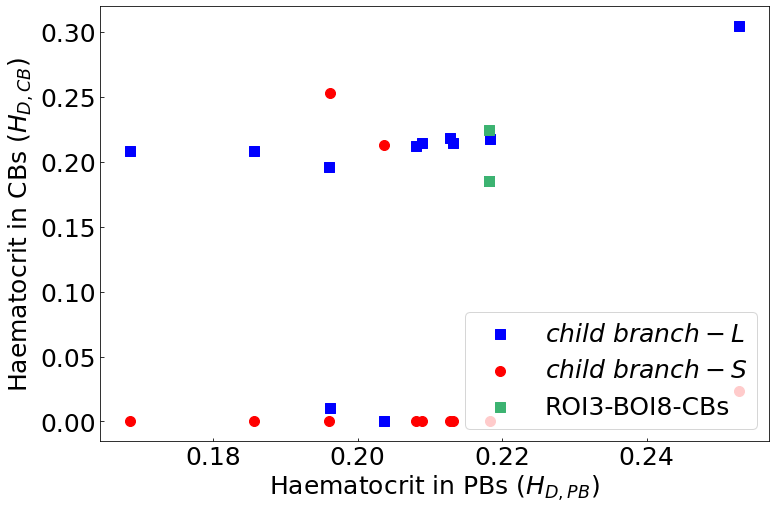
\includegraphics[width=0.6\textwidth]{images/DownstreamBifurcationHD.png}
\caption{\textit{Large haematocrit difference between the "L" and "S" child branches in each downstream bifurcation. The "L"/"S" indicate the relatively larger (blue squares) and smaller (red circles) child branches in each diverging bifurcation respectively. The green squares indicate the anomaly among all of the identified successive bifurcations.} \label{DownstreamBifurcationHD}}
\end{figure}

\noindent It was found that due to the primary assumption of axisymmetric RBC distribution in the parent branch for the empirical formulation of PSM\cite{A.R.Pries2005Mbvi, PriesAR1990BFiM}, inaccuracies will emerge when applying PSM to successive bifurcations instead of individual bifurcations across the networks. This has been demonstrated by first identifying the successive bifurcations found from simulation data (see Table \ref{SuccessiveBOIs} for the complete list) and afterwards observing the change in RBC concentration (i.e. haematocrit) in the downstream bifurcations. From Figure \ref{DownstreamBifurcationHD}, the majority of the downstream bifurcations were found to have a significantly large haematocrit difference between the child branches regardless of high or low haematocrit in the parent branches. Only one successive bifurcation (ROI3: BOI-7 $\Rightarrow$ BOI-8) indicated in green had a small haematocrit difference between the child branches of the downstream bifurcation. This features the emerging heterogeneity of RBC partitioning in successive bifurcations as the simulated RBC fluxes substantially deviate from PSM's empirical predictions. An explanation for this phenomenon was suggested by a recent study\cite{Zhou2021EmergentBifurcations} where the excessive heterogeneity is attributed to the lack of symmetrical cell-free layer (CFL) recovery in the inter-bifurcation branches. Therefore, the upstream deviations in the CFL can naturally lead to child branches deprived of RBCs even for equal blood flow split. 

% \begin{figure}[H]
% \centering
% \begin{subfigure}{0.48 \textwidth}
%     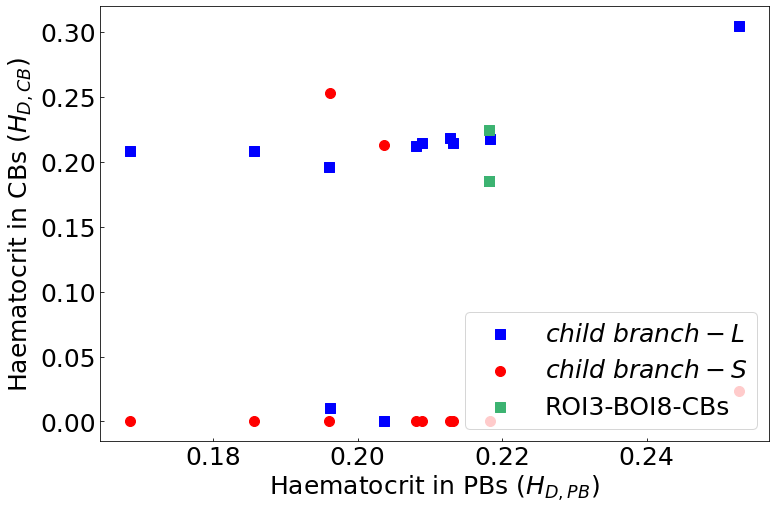
\includegraphics[width=1\textwidth]{images/DownstreamBifurcationHD.png}
%     \caption{\textit{Large haematocrit difference between the child branches of downstream bifurcations} \label{DownstreamBifurcationHD}}
% \end{subfigure}
% \hfill
% \begin{subfigure}{0.48 \textwidth}
%     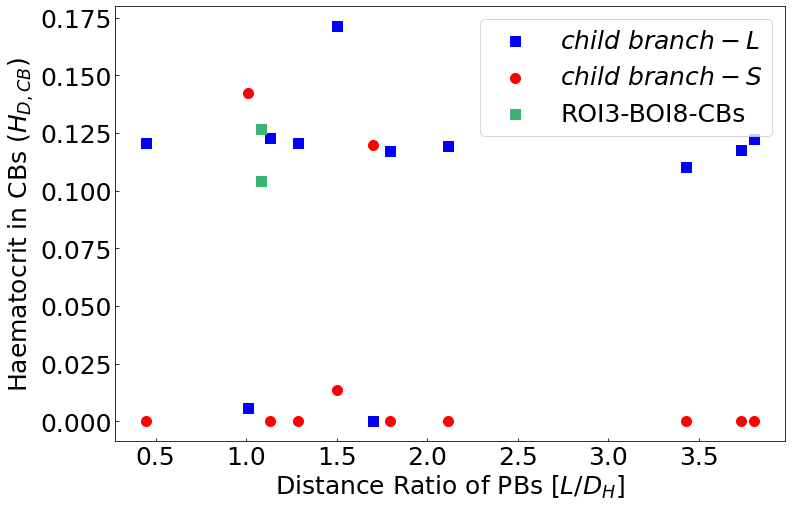
\includegraphics[width=1\textwidth]{images/DownstreamBifurcationDL.png}
%     \caption{\textit{Evaluated Hydrodynamic Diameters} \label{DownstreamBifurcationDL}}
% \end{subfigure}
% \caption{\textit{} \label{DownstreamBifurcations}}
% \end{figure}